\documentclass{standalone}
\usepackage{tikz}
\usetikzlibrary{arrows.meta, positioning, fit, backgrounds}

\begin{document}
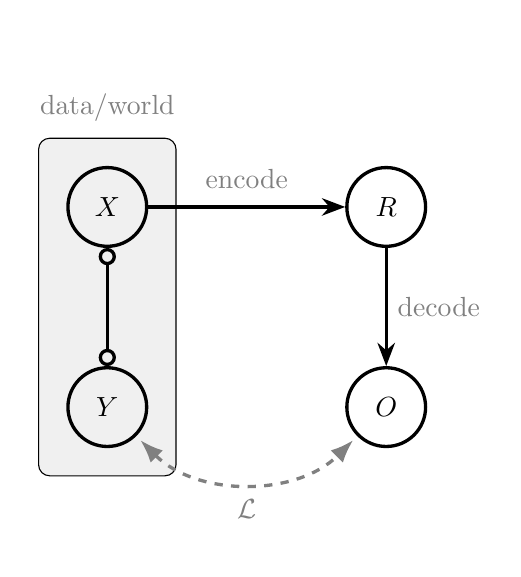
\begin{tikzpicture}[>=Stealth, line width=1.2pt, every node/.style={draw, circle, minimum size=1cm}]


  % Nodes
  \node (Y) {$Y$};
  \node (X) [above=1.5cm of Y] {$X$};
  \node (R) [right=2.5cm of X] {$R$};
  \node (O) [below=1.5cm of R] {$O$};

  % Background rectangle
  \begin{scope}[on background layer]
    \node[draw, rectangle, rounded corners, fill=gray!12, inner sep=10pt,
          fit=(X)(Y), label={[draw=none, text=gray, label distance=-18pt]north:data/world}] {};
  \end{scope}

  % Edges
  \draw[{Circle[open]}-{Circle[open]}] (X)  -- (Y);
  \draw[->] (X)  -- node[midway, above=-10pt, draw=none] {\textcolor{gray}{encode}} (R);
  \draw[->] (R)  -- node[midway, right=-1pt, draw=none] {\textcolor{gray}{decode}} (O);
  \draw[{Latex}-{Latex}, gray, dashed, shorten <=2pt, shorten >=2pt]
  (Y) to[out=-45, in=-135]
  node[midway, below=-5pt, draw=none] {$\mathcal{L}$}
  (O);

\end{tikzpicture}
\end{document}
